\documentclass[11pt]{article}

\usepackage[T1]{fontenc}
\usepackage{geometry}
\usepackage{amsmath, amssymb, amsthm}
\usepackage{bm}
\usepackage[scr]{rsfso}
\usepackage{graphicx}
\usepackage{float}
\usepackage{xcolor}
\usepackage{hyperref}

\geometry{a4paper, margin=1in, headheight=14pt}

\renewcommand{\labelenumi}{(\alph{enumi})}
\renewcommand{\labelenumii}{(\roman{enumii})}

\def\C{\mathbb{C}}
\def\R{\mathbb{R}}
\def\Q{\mathbb{Q}}
\def\Z{\mathbb{Z}}
\def\N{\mathbb{N}}

\newtheorem{theorem}{Theorem}[section]
\newtheorem{corollary}{Corollary}[theorem]
\newtheorem{lemma}[theorem]{Lemma}

\theoremstyle{definition}
\newtheorem{definition}{Definition}[section]

\theoremstyle{remark}
\newtheorem*{remark}{Remark}
\newtheorem*{example}{Example}

\title{
    \Large\textsc{Summer Programme 2021} \\
    \vspace{10pt}
    \textit{\Large Approximating continuous functions by smooth functions:} \\
    \vspace{6pt}
    {\huge\bf The Stone-Weierstrass Theorem}
}
\author{
    \large Satvik Saha%
    % \thanks{Email: \tt ss19ms154@iiserkol.ac.in}
    \\\textsc{\small 19MS154}
}
\date{\normalsize
    \textit{Indian Institute of Science Education and Research, Kolkata, \\
    Mohanpur, West Bengal, 741246, India.} \\
    % \vspace{10pt}
    % \today
}


\begin{document}
    \maketitle

    \section{Sequences of functions}
    \begin{definition}
        Let $\{f_n\}$ be a sequence of functions on a set $E$. We say that
        $\{f_n\}$ converges \textit{pointwise} to a function $f$ on $E$ if the
        sequences $f_n(x) \to f(x)$ for every $x \in E$. We write $f_n \to f$
        pointwise on $E$.
    \end{definition}

    \begin{definition}
        Let $\{f_n\}$ be a sequence of functions on a set $E$. We say that
        $\{f_n\}$ converges \textit{uniformly} to a function $f$ on $E$ if given
        $\epsilon > 0$, there exists $n_0 \in \N$ such that $d(f_n(x), f(x)) <
        \epsilon$ for all $x \in E$, $n \geq n_0$.  We write $f_n \to
        f$ uniformly on $E$.
    \end{definition}

    \begin{lemma}
        Let $\mathscr{G}$ be a collection of functions on a set $E$, and let
        $f$ be a function on $E$ with the following property: given $\epsilon >
        0$, there exists $g \in \mathscr{G}$ such that $|g(x) - f(x)| <
        \epsilon$ for all $x \in E$. Then, $f$ is the uniform limit of functions in
        $\mathscr{G}$.
    \end{lemma}
    \begin{proof}
        For all $n \in \N$, let $g_n \in \mathscr{G}$ be the function such that
        $|g_n(x) - f(x)| < 1 / n$ for all $x \in E$.  Then, $g_n \to f$ uniformly on
        $E$. To prove this, let $\epsilon > 0$. Using the Archimedean property of the
        reals, pick $n_0 \in \N$ such that $n_0\epsilon > 1$. Thus, for all $x \in E$
        and $n \geq n_0$, we have \[
            |g_n(x) - f(x)| < \frac{1}{n} \leq \frac{1}{n_0} < \epsilon. \qedhere
        \] 
    \end{proof}

    \begin{theorem}[Cauchy criterion] \label{theo:cauchy_criterion}
        Let $\{f_n\}$ be a sequence of real valued functions on a set $E$.
        This sequence of functions converges uniformly on $E$ if and only if given
        $\epsilon > 0$, there exists $n_0 \in \N$ such that \[
            |f_n(x) - f_m(x)| < \epsilon
        \] for all $x \in E$, $m, n \geq n_0$.
    \end{theorem} 
    \begin{proof}
        First, suppose that the sequence of real valued functions $\{f_n\}$ converges
        uniformly on $E$, with $f_n \to f$ uniformly. Given $\epsilon > 0$, we choose
        $n_0 \in \N$ such that for all $x \in E$ and $n \geq n_0$, \[
            |f_n(x) - f(x)| < \frac{\epsilon}{2}.
        \] Now, for all $x \in E$ and $m, n \geq n_0$, we have
        \begin{align*}
            |f_n(x) - f_m(x)| &= |(f_n(x) - f(x)) - (f_m(x) - f(x))| \\
            &\leq |f_n(x) - f(x)| + |f_m(x) - f(x)| \\
            & < \frac{\epsilon}{2} + \frac{\epsilon}{2} \\
            &= \epsilon.
        \end{align*}
        Thus, $\{f_n\}$ is a Cauchy sequence.

        Next, suppose that $\{f_n\}$ is a Cauchy sequence. Given $\epsilon > 0$,
        choose $n_0 \in \N$ such that for all $x \in E$ and $m, n \geq 0$, we have \[
            |f_n(x) - f_m(x)| < \frac{\epsilon}{2}.
        \] Now for each point $x \in E$, the Cauchy criterion for convergence of a
        sequence of real numbers guarantees that $\lim_{n \to \infty} f_n(x)$ exists.
        Thus, we can define the function $f$ on $E$ such that $f(x) = \lim_{n \to
        \infty} f_n(x)$, hence $f_n \to f$ pointwise. Fix $x_0 \in E$, and pick $n_0'
        \in \N$ such that for all $m \geq n_0'$, we have $|f_m(x_0) - f(x_0)| <
        \epsilon / 2$. Choose $m = \max(n_0, n_0')$, whence for all $n \geq n_0$, we
        have
        \begin{align*}
            |f_n(x_0) - f(x_0)| &= |(f_n(x_0) - f_m(x_0)) + (f_m(x_0) - f(x_0))| \\
            &\leq |f_n(x_0) - f_m(x_0)| + |f_m(x_0) - f(x_0)| \\
            &\leq \frac{\epsilon}{2} + \frac{\epsilon}{2} \\
            &= \epsilon.
        \end{align*}
        Note that $x_0$ was arbitrary, with $n_0$ chosen independently of $x_0$.
        Thus, $\{f_n\}$ converges uniformly on $E$.
    \end{proof}
    
    \begin{theorem} \label{theo:uniform_M_n}
        Let $\{f_n\}$ be a sequence of real valued functions on a set $E$,
        and let $f$ be a real valued function on $X$ such that $f_n \to f$ pointwise.
        For all $n \in \N$, set \[
            M_n = \sup_{x \in E} |f_n(x) - f(x)|
        \] Then, $f_n \to f$ uniformly on $E$ if and only if $M_n \to 0$.
    \end{theorem}
    \begin{proof}
        First, suppose that $M_n \to 0$. This means that given $\epsilon > 0$, we can
        find $n_0 \in \N$ such that for all $n \geq n_0$, we have \[
            M_n = \sup_{n \in X}|f_n(x) - f(x)| < \epsilon.
        \] This directly gives \[
            |f_n(x) - f(x)| \leq \sup_{x \in X}|f_n(x) - f(x)| < \epsilon
        \] for all $x \in E$ and $n \geq n_0$, hence $f_n \to f$ uniformly on $E$.

        Next, suppose that $f_n \to f$ uniformly on $E$. Let $\epsilon > 0$ and pick
        $n_0 \in \N$ such that for all $x \in E$ and $n \geq n_0$, we have $|f_n(x) -
        f(x)| < \epsilon / 2$. Taking supremums gives \[
            M_n = \sup_{x \in E}|f_n(x) - f(x)| \leq \frac{\epsilon}{2} < \epsilon,
        \] hence $M_n \to 0$.
    \end{proof}

    \begin{theorem} \label{theo:uniform_bounded}
        Let $\{f_n\}$ be a sequence of real valued bounded, functions on a set $E$,
        and let $f$ be a function on $E$ such that $f_n \to f$ uniformly.  Then, $f$
        is bounded on $E$.
    \end{theorem}
    \begin{proof}
        Using the uniform convergence of $\{f_n\}$, choose $n_0 \in \N$ such that \[
            |f_n(x) - f(x)| < 1
        \] for all $x \in E$ and $n \geq n_0$. Specifically, this holds for $n =
        n_0$ so for all $x \in E$, we have \[
            f_n(x) - 1 < f(x) < f_n(x) + 1.
        \] However, $f_n$ is bounded so there exists $M > 0$ such that $|f_n(x)| < M$
        for all $x \in E$, hence \[
            -M - 1 < f(x) < M + 1
        \] or $|f(x)| < M + 1$ for all $x \in E$.
    \end{proof}

    \begin{theorem}[Uniform limit theorem] \label{theo:uniform_limit}
        Let $\{f_n\}$ be a sequence of continuous functions on a metric space $X$,
        and let $f$ be a function on $X$ such that $f_n \to f$ uniformly. Then, $f$
        is continuous on $X$.
    \end{theorem}
    \begin{proof}
        Fix $x_0 \in X$, and let $\epsilon > 0$.
        Use the uniform convergence of $\{f_n\}$ to pick $n_0 \in \N$ such that for
        all $x \in X$ and $n \geq n_0$, \[
            |f_n(x) - f(x)| < \frac{\epsilon}{3}.
        \] Note that the above also holds specifically at $x = x_0$.
        Use the continuity of each $f_n$ to choose $\delta > 0$ such that for all $x
        \in X$ satisfying $|x - x_0| < \delta$, we have \[
            |f_n(x_0) - f_n(x)| < \frac{\epsilon}{3}.
        \] Set $n = n_0$, whence for all $x \in X$ satisfying $|x - x_0| < \delta$,
        we have
        \begin{align*}
            |f(x_0) - f(x)| &= |(f(x_0) - f_n(x_0)) + (f_n(x_0) - f_n(x)) + (f_n(x)
            - f(x))| \\
            &\leq |f(x_0) - f_n(x_0)| + |f_n(x_0) - f_n(x)| + |f_n(x) - f(x)| \\
            &\leq \frac{\epsilon}{3} + \frac{\epsilon}{3} + \frac{\epsilon}{3} \\
            &= \epsilon.
        \end{align*}
        Thus, $f$ is continuous at $x_0$. Since $x_0$ was chosen arbitrarily, $f$ is
        continuous on $X$.
    \end{proof}

    \begin{theorem}[Dini's theorem] \label{theo:dini}
        Let $\{f_n\}$ be a sequence of continuous real valued functions on a compact
        metric space $K$ such that $f_n \geq f_{n + 1}$ for all $n \in \N$, and let
        $f$ be a continuous function on $K$ such that $f_n \to f$ pointwise. Then,
        $f_n \to f$ uniformly on $K$.
    \end{theorem}
    \begin{proof}
        Let $\epsilon > 0$. For each $n \in \N$, set $g_n = f_n - f$ and note that
        the each $g_n$ is continuous, with $g_n \geq g_{n + 1}$ and $g_n \to 0$
        pointwise on $K$. Since $\{g_n\}$ is a decreasing sequence, we must have $g_n
        \geq 0$ for all $n \in \N$.  It is sufficient to show that $g_n \to 0$
        uniformly on $K$, i.e.\ there exists $n_0 \in \N$ such that for all $x \in K$
        and $n \geq n_0$, we have $g_n(x) < \epsilon$.

        Define the sets \[
            G_n = g_n^{-1}[\epsilon, \infty) = \{x \in K\colon g_n(x) \geq \epsilon\}.
        \] Since each $g_n$ is continuous, the sets $G_n$ which are the pre-images of
        closed sets in $\R$ are closed. Furthermore, $G_n$ is the intersection of the
        closed set $G_n$ and the compact set $K$, hence each $G_n$ is compact. Note
        that if $x \in G_{n + 1}$ for some $n \in \N$, then $g_{n + 1}(x) \geq
        \epsilon \implies g_n(x) \geq g_{n + 1}(x) \geq \epsilon$ so $x \in G_n$;
        this means that $G_n \supseteq G_{n + 1}$ for all $n \in \N$. Thus, if any
        $G_{n_0}$ happened to be empty, then all subsequent $G_{n \geq n_0} =
        \emptyset$ as well.

        Suppose that all $G_n$ are non-empty. Then the countable intersection of
        nested compact sets $G = \bigcap_{n \in \N} G_n$ must also be non-empty. Pick
        $x_0 \in G$, and note that $x_0 \in G_n$ for all $n \in \N$, which means
        $g_n(x_0) \geq \epsilon$ for all $n \in \N$. This contradicts the fact that
        $g_n(x_0) \to 0$ pointwise. Thus, there must be some $G_{n_0} = \emptyset$,
        hence $G_{n \geq n_0} = \emptyset$. In other words, for all $n \geq n_0$,
        there is no $x \in K$ such that $g_n(x) \geq \epsilon$. This completes the
        proof.
    \end{proof}
    \begin{remark}
        Note that the continuity of $f$, the compactness of $K$, and the monotonicity
        of $\{f_n\}$ are all essential.
        \begin{enumerate}
            \item Consider $f_n\colon [0, 1] \to \R$, $x \mapsto x^n$, and note that
            $x^n \geq x^{n + 1}$ on $[0, 1]$. We have $f_n \to f$ pointwise on the
            compact interval $[0, 1]$, where \[
                f\colon [0, 1]\to \R, \qquad x \mapsto \begin{cases}
                    0, &\text{ if }0 \leq x < 1, \\
                    1, &\text{ if }x = 1.
                \end{cases}
            \] However, $f$ is not continuous, and indeed $f_n \not\to f$ uniformly
            on $[0, 1]$ by the contrapositive of Theorem~\ref{theo:uniform_limit}.
            
            \item Consider $f_n\colon (0, 1) \to \R$, $x \mapsto x^n$, with $x^n \geq
            x^{n + 1}$. We have $f_n \to 0$ pointwise on the open interval $(0, 1)$.
            However, $(0, 1)$ is not compact, and indeed $f_n \not\to 0$ uniformly on
            $(0, 1)$. Note that $0 < 2^{-1 / n} < 1$ for all $n \in \N$, and
            $f_n(2^{-1 / n}) = 1 / 2$. Thus, there is no $n_0 \in \N$ such that
            $|f_n(x)| < 1 / 4$ for all $n \geq n_0$.

            \item Consider the triangular spike functions \[
                f_n\colon [0, 1] \to \R, \qquad x \mapsto \begin{cases}
                    nx, &\text{ if } 0 \leq x \leq 1 / 2n, \\
                    1 - nx, &\text{ if } 1 /2n < x \leq 1 / n, \\
                    0, &\text{ if } 1 / n < x \leq 1.
                \end{cases}
            \] Note that $f_n \to 0$ pointwise on the compact interval $[0, 1]$,
            because given any $x_0 \in (0, 1]$, we can choose sufficiently large $n_0
            \in \N$ such that $n_0x_0 > 1$, hence $f_n(x_0) = 0$ for all $n \geq
            n_0$; if $x_0 = 0$, then $f_n(0) = 0$ for all $n \in \N$ anyway. However,
            the sequence $\{f_n\}$ is not monotonic, and indeed this convergence is
            not uniform on $[0, 1]$. Note that $f_n(1 / 2n) = 1 / 2$ for all $n \in
            \N$, hence $\sup |f_n(x)| \geq 1 / 2 \not\to 0$.
        \end{enumerate}
    \end{remark}

    \section{The Weierstrass Approximation Theorem}
    \begin{definition}[Bernstein polynomials]
        The Bernstein polynomial $B_n^k(x)$ for integers $0 \leq k \leq n$ is defined
        as \[
            B_n^k(x) = \binom{n}{k} x^k (1 - x)^{n - k}.
        \] 
    \end{definition}
    \begin{remark}
        Each polynomial $B_n^k$ on the interval $[0, 1]$ peaks at $x = k / n$. See
        Figure~\ref{fig:bernstein_7}.
    \end{remark}
    \begin{figure}
        \centering
        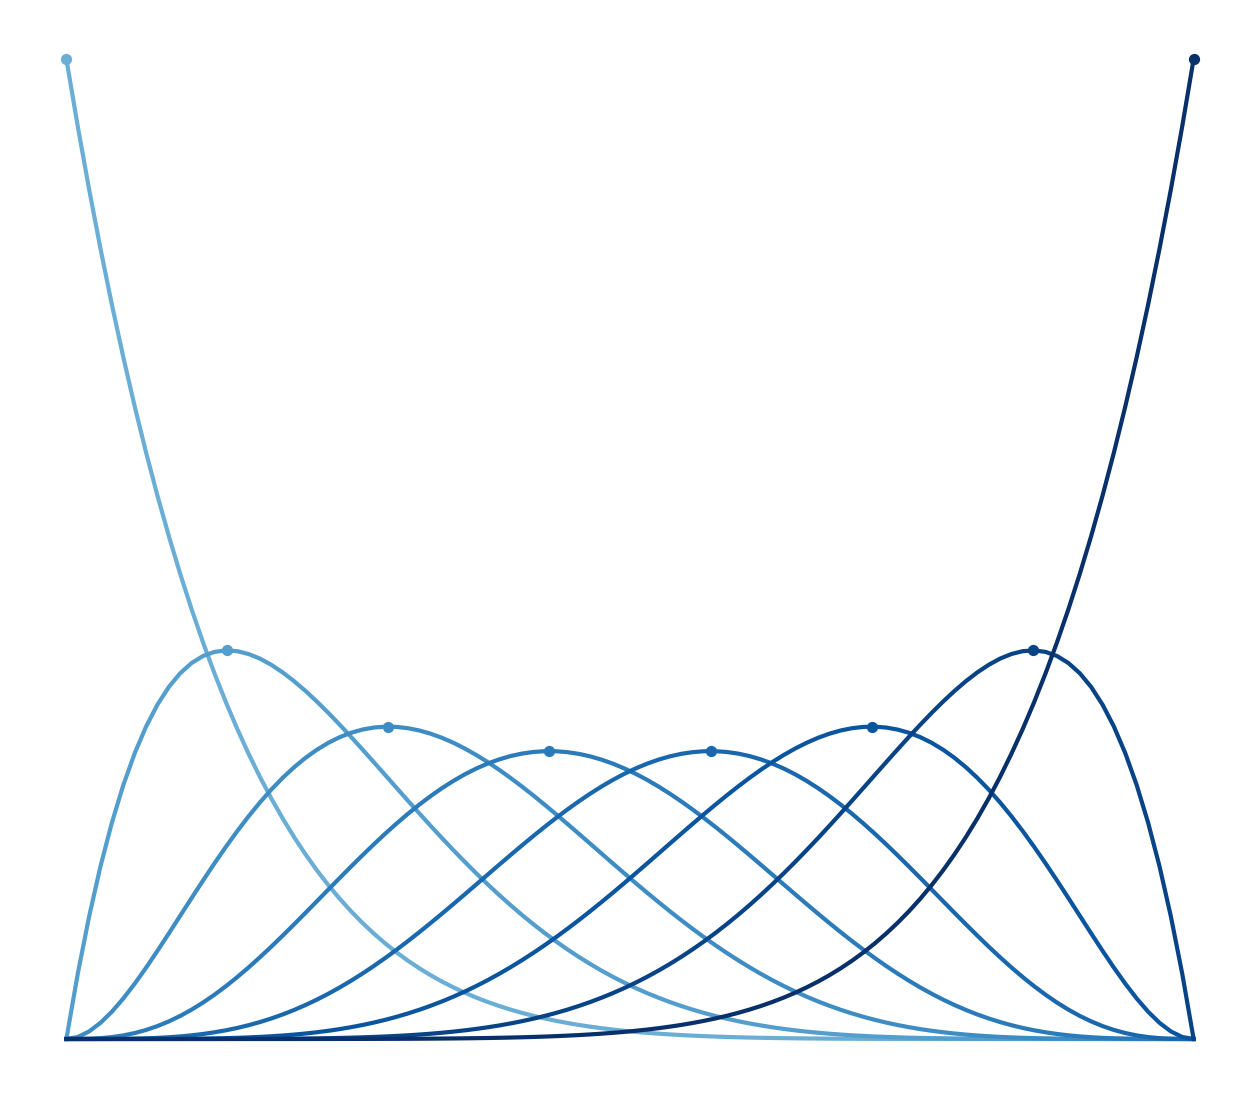
\includegraphics[width=0.75\textwidth]{./img/bernstein_7.png}
        \caption{The Bernstein polynomials of degree $7$. The peaks at $x = k / 7$ have
        been marked.}
        \label{fig:bernstein_7}
    \end{figure}

    \begin{definition}[Bernstein expansions]
        Let $f$ be a real valued function on $[0, 1]$. The Bernstein polynomial
        expansion of $f$ is defined as \[
            B_n(f, x) = \sum_{k = 0}^n \binom{n}{k} x^k(1 - x)^{n - k}f\left(
            \frac{k}{n} \right).
        \]
    \end{definition}

    \begin{figure}[t]
        \centering
        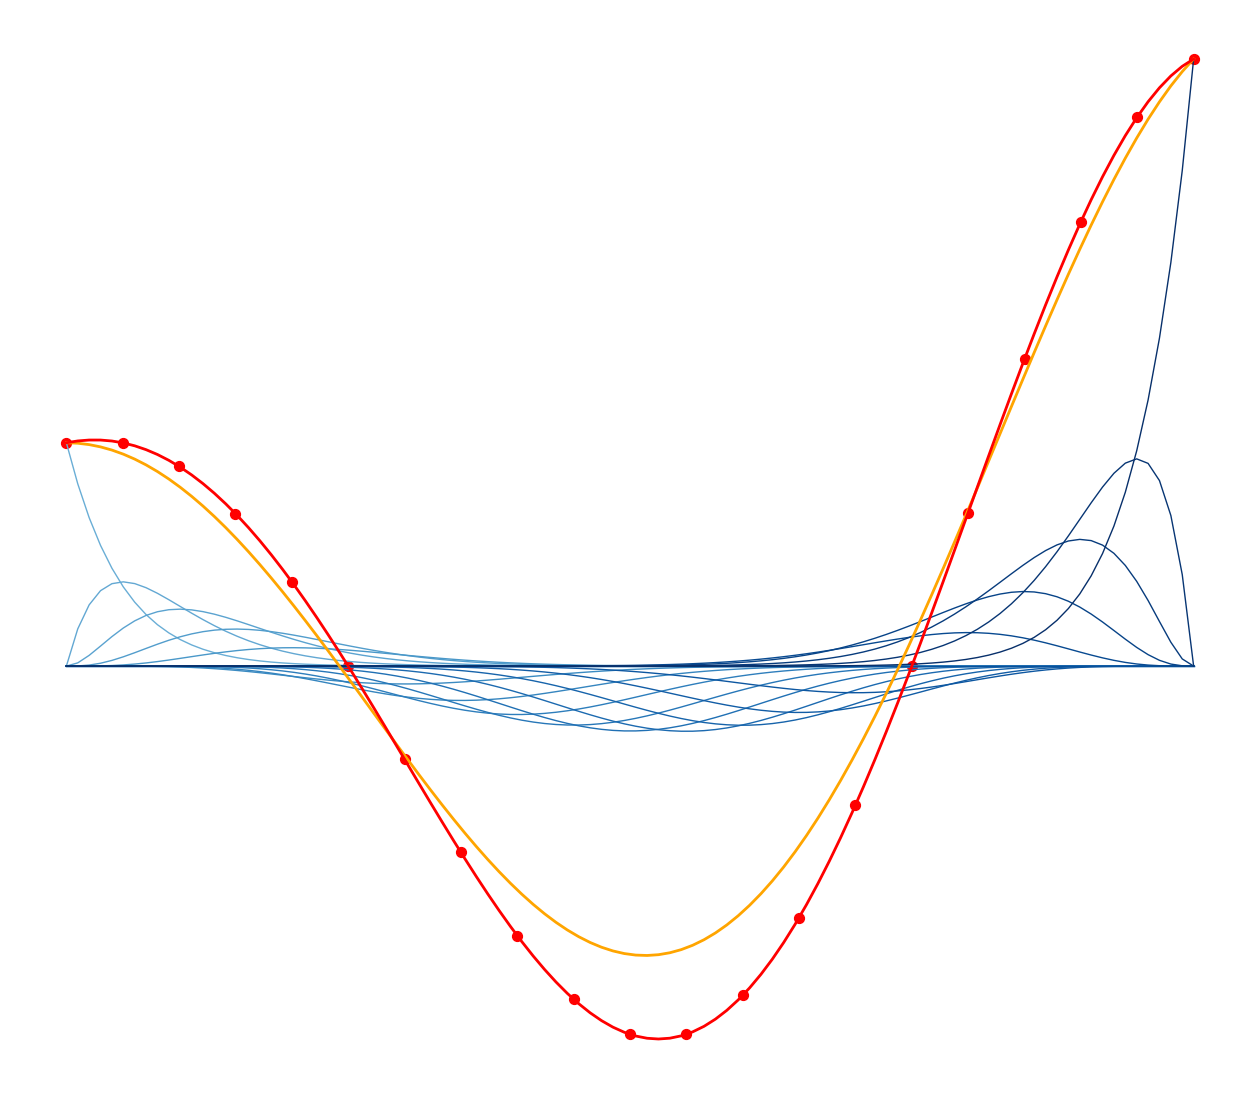
\includegraphics[width=0.9\textwidth]{./img/expansion_20.png}
        \caption{The Bernstein polynomial expansion of order $20$ (orange) of the
        curve $f(x) = e^x\cos(2\pi x)$ (red) on $[0, 1]$. Each term of the sum has
        been shown in blue. Note that only the marked points at $x = k / 20$ have
        been sampled from $f$.}
        \label{fig:expansion_20}
    \end{figure}

    \begin{lemma}
        The following identities hold. \[
            B_n(1, x) = 1, \qquad B_n(x, x) = x, \qquad B_n(x^2, x) = \frac{x}{n} +
            \frac{n - 1}{n}x^2.
        \] 
    \end{lemma}
    \begin{proof}
        The Binomial Theorem gives the expansion \[
            (x + y)^n = \sum_{k = 0}^n \binom{n}{k} x^k y^{n - k}.
        \] Taking a partial derivative with respect to $x$ and multiplying by $x/n$, we
        have
        \begin{align*}
            n(x + y)^{n - 1} &= \sum_{k = 0}^n \binom{n}{k} kx^{k - 1} y^{n - k}, \\
            x(x + y)^{n - 1} &= \sum_{k = 0}^n \binom{n}{k} x^k y^{n - k}
            \left( \frac{k}{n} \right).
        \end{align*}
        Repeating the same procedure, we have
        \begin{align*}
            (x + y)^{n - 1} + (n - 1)x(x + y)^{n - 2} &= \sum_{k = 0}^n \binom{n}{k}
            kx^{k - 1} y^{n - k} \left( \frac{k}{n} \right), \\
            \frac{x}{n}(x + y)^{n - 1} + \frac{n - 1}{n}x^2(x + y)^{n - 2} &= \sum_{k
            = 0}^n \binom{n}{k} x^k y^{n - k} \left( \frac{k}{n} \right)^2.
        \end{align*}
        Finally, set $y = 1 - x$ upon which all $x + y$ terms become $1$ and the
        right hand sides become the Bernstein expansions of $1$, $x$, and $x^2$. This
        establishes the desired identities.
    \end{proof}
    
    \begin{theorem}
        Let $f$ be a real valued continuous function on the closed interval $[0, 1]$,
        and let $\epsilon > 0$. There exists a polynomial $p$ such that $|p(x) -
        f(x)| < 0$ on $x \in [0, 1]$.
    \end{theorem}
    \begin{proof} \label{theo:weierstrass}
        We claim that a Bernstein polynomial expansion $B_n(f, x)$ of sufficiently
        high order satisfies the given conditions. Let $\epsilon > 0$.  Now, the
        continuity of $f$ on the compact interval $[0, 1]$ implies that it is
        uniformly continuous and bounded. Thus, there exists $\delta > 0$ such that
        whenever $|x - x_0| < \delta$ for $x, x_0 \in [0, 1]$, we have \[
            |f(x) - f(x_0)| < \frac{\epsilon}{2}.
        \] Fix $x_0 \in [0, 1]$. Observe that $M = \sup_{x \in [0, 1]} |f(x)|$ is
        finite. Thus, in those cases where $|x - x_0| \geq \delta$, use $|x - x_0| /
        \delta \geq 1$ and the triangle inequality to write \[
            |f(x) - f(x_0)| \leq 2M \leq 2M \left(\frac{x - x_0}{\delta}\right)^2.
        \] Thus, for all $x \in [0, 1]$ we have \[
            |f(x) - f(x_0)| \leq 2M \left(\frac{x - x_0}{\delta}\right)^2 +
            \frac{\epsilon}{2}.
        \]
        Write
        \begin{align*}
            B_n(f, x) - f(x_0) &= B_n(f, x) - B_n(1, x)\,f(x_0) \\
            &= \sum_{k = 0}^n \binom{n}{k} x^k(1 - x)^{n - k}f \left(
            \frac{k}{n} \right) - \sum_{k = 0}^n \binom{n}{k} x^k(1 - x)^{n - k}f(x_0)
            \\
            &= \sum_{k = 0}^n \binom{n}{k} x^k(1 - x)^{n - k}\left[ f\left(
            \frac{k}{n} \right) - f(x_0)\right].
        \end{align*}
        The triangle inequality, followed by our estimate of $|f(x) - f(x_0)|$, gives 
        \begin{align*}
            |B_n(f, x) - f(x_0)| &\leq \sum_{k = 0}^n \binom{n}{k} x^k(1 - x)^{n -
            k}\left| f\left( \frac{k}{n} \right) - f(x_0)\right| \\
            &\leq \sum_{k = 0}^n \binom{n}{k} x^k(1 - x)^{n -
            k}\left[ 2M\left(\frac{k / n - x_0}{\delta}\right)^2 + \frac{\epsilon}{2}
            \right] \\
            &= \frac{2M}{\delta^2} B_n((x - x_0)^2, x) + \frac{\epsilon}{2} \\
            &= \frac{2M}{\delta^2} \left[B_n(x^2, x) - 2x_0B_n(x, x) + x_0^2\right] +
            \frac{\epsilon}{2} \\
            &= \frac{2M}{\delta^2}\left[\frac{x}{n} + x^2 - \frac{x^2}{n} - 2xx_0 +
            x_0^2\right] + \frac{\epsilon}{2}.
        \end{align*}
        The term in square brackets can be rearranged as \[
            (x - x_0)^2 + \frac{1}{n}(x - x^2).
        \] Use $(x - 1 / 2)^2 \geq 0$ to conclude that $x - x^2 \leq 1 / 4$, and
        evaluate the expression at $x = x_0$ to write \[
            |B_n(f, x_0) - f(x_0)| \leq \frac{M}{2n\delta^2} + \frac{\epsilon}{2}.
        \] Therefore, setting $n_0 > M / 2\epsilon\delta^2$, we see that \[
            |B_{n_0}(f, x_0) - f(x_0)| < \epsilon.
        \] Since $x_0 \in [0, 1]$ was arbitrary, this concludes the proof.
    \end{proof}
    
    \begin{figure}[ht]
        \centering
        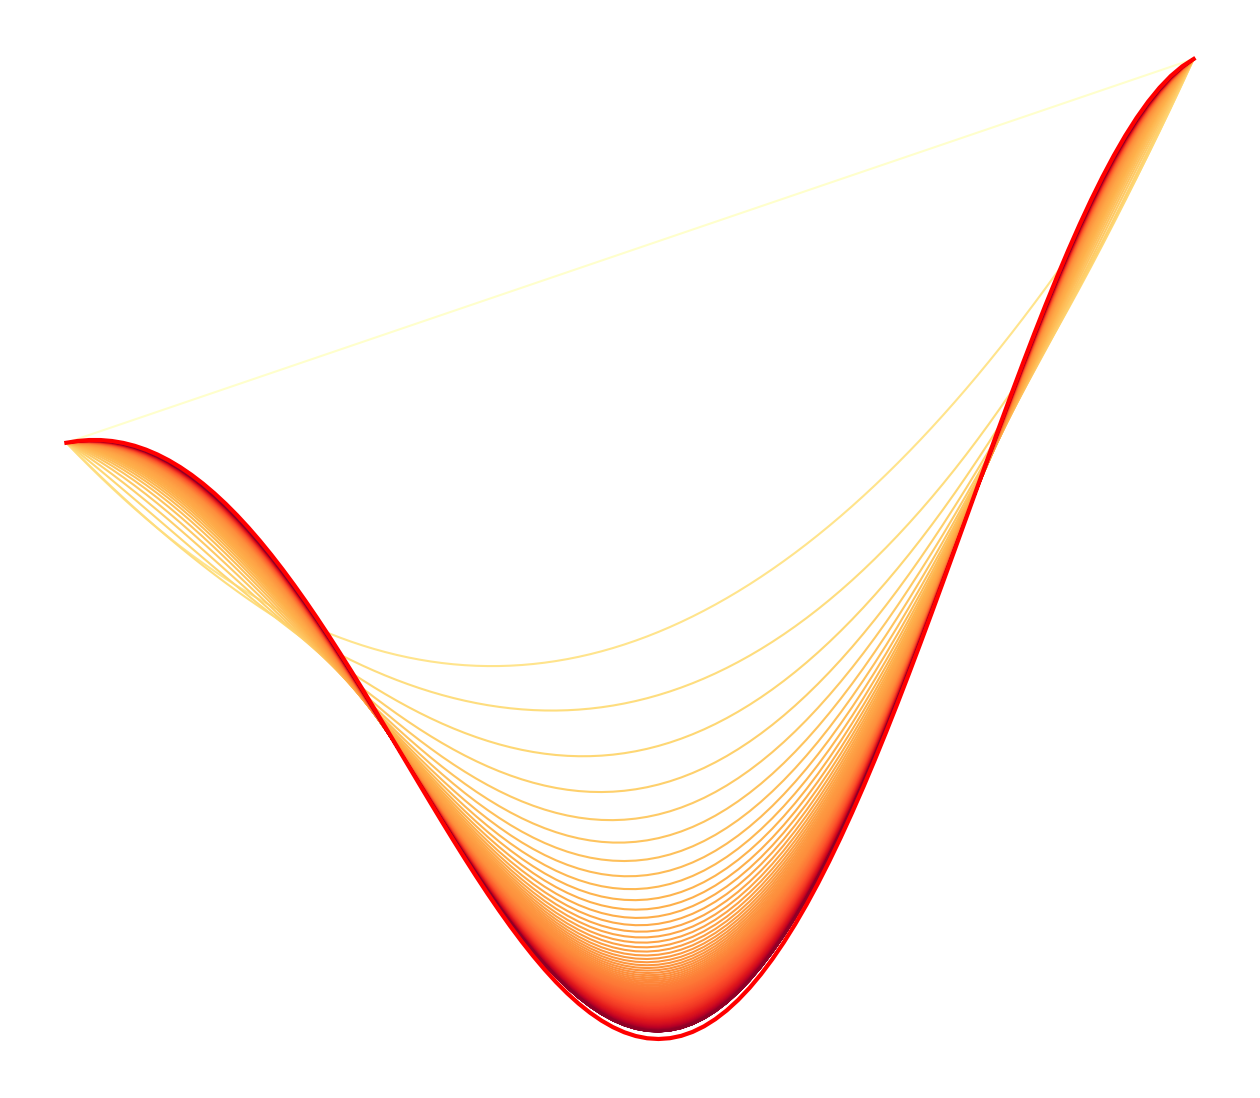
\includegraphics[width=0.9\textwidth]{./img/expansions.png}
        \caption{The first 250 Bernstein expansions of $e^x\cos(2\pi x)$ on $[0, 1]$.
        Note that convergence is fairly slow.}
        \label{fig:expansion}
    \end{figure}

    \begin{corollary}
        Given any real valued continuous function $f$ on $[0, 1]$, there exists a
        sequence of polynomials $\{p_n\}$ such that $p_n \to f$ uniformly on $[0,
        1]$.
    \end{corollary}
    \begin{corollary}
        The same holds for any real valued continuous function on some closed interval
        $[a, b]$.
    \end{corollary}
    \begin{proof}
        Consider the continuous bijection \[
            \varphi\colon [0, 1] \to [a, b], \qquad x \mapsto (b - a)x + a.
        \] For an arbitrary real valued continuous function $f\colon [a, b] \to \R$,
        note that the composition $g = f\circ \varphi$ is also continuous with domain
        $[0, 1]$. Given $\epsilon > 0$, we find a polynomial $p$ such that \[
            |p(x) - f(\varphi(x))| = |p(x) - g(x)| < \epsilon
        \] on $[0, 1]$, which means that \[
            |p(\varphi^{-1}(x)) - f(x)| < \epsilon
        \] on $[a, b]$. Now, $\varphi^{-1}(x) = (x - a) / (b - a)$, hence $p \circ
        \varphi^{-1}$ is also a polynomial, as desired.
    \end{proof}


    \section{Metric spaces of continuous functions}
    \begin{theorem}
        Let $X$ be a metric space and let $\mathscr{C}(X)$ denote the set of all
        real valued, continuous, bounded functions on $X$. Define the distance function \[
            d(f, g) = \sup_{x\in X} |f(x) - g(x)|
        \] for all $f, g \in \mathscr{C}(X)$. Then, $\mathscr{C}(X)$ is a metric space.
    \end{theorem}
    \begin{proof}
        Let $f, g, h\in \mathscr{C}(X)$ be arbitrary. The non-negativity of $d(f, g)$ is
        evident since it is the supremum of non-negative quantities. Furthermore, $f$
        and $g$ are bounded so $d(f, g) = \sup |f - g| \leq \sup |f| + \sup |g|$ is
        finite. We clearly have $d(f, f) = 0$; conversely, if $d(f, g) = 0$, then
        $0 \leq \sup |f - g| = 0$ forcing $|f(x) - g(x)| = 0$ on $X$, hence $f = g$.
        Symmetry of $d$ is evident from the fact that $|f(x) - g(x)| = |g(x) - f(x)|$
        everywhere, hence $d(f, g) = d(g, f)$. Finally, the triangle inequality gives
        \[
            |f(x) - h(x)| \leq |f(x) - g(x)| + |g(x) - h(x)|,
        \] whence taking supremums immediately gives $d(f, h) \leq d(f, g) + d(g,
        h)$.
    \end{proof}

    \begin{theorem}
        The metric space $\mathscr{C}(X)$ is complete.
    \end{theorem}
    \begin{proof}
        We claim that every Cauchy sequences in $\mathscr{C}(X)$ converges in
        $\mathscr{C}(X)$

        Let $\{f_n\}$ be a Cauchy sequence in $\mathscr{C}(x)$. Given any $\epsilon >
        0$ we can find $n_0 \in \N$ such that for all $m, n \geq n_0$, $d(f_n, f_m) <
        \epsilon$. Thus, \[
            |f_n(x) - f_m(x)| \leq \sup_{x \in X} |f_n(x) - f_m(x)| = d(f_n, f_m)<
            \epsilon
        \] for all $x \in X$ and $m, n \geq n_0$, hence
        Theorem~\ref{theo:cauchy_criterion} says that $f_n \to f$ uniformly on $X$.
        Theorem~\ref{theo:uniform_M_n} says that $d(f_n, f) \to 0$.  Since each $f_n$
        is bounded and continuous, Theorems~\ref{theo:uniform_bounded} and
        \ref{theo:uniform_limit} guarantee that $f$ is also bounded and continuous.
        Thus, $f \in \mathscr{C}(X)$, hence the Cauchy sequence $\{f_n\}$ converges
        in $\mathscr{C}(X)$.
    \end{proof}

    \section{Algebras of functions}
    \begin{definition}
        A family $\mathscr{A}$ of real valued functions on a set $E$ is called an
        algebra if $f + g \in \mathscr{A}$, $fg \in \mathscr{A}$, and $cf \in
        \mathscr{A}$ for all $f, g\in \mathscr{A}$ and $c \in \R$.
    \end{definition}

    \begin{definition}
        An algebra $\mathscr{A}$ is uniformly closed if given any sequence of
        functions $\{f_n\}$ in $\mathscr{A}$ such that $f_n \to f$ uniformly, we have
        $f \in \mathscr{A}$.
    \end{definition}

    \begin{definition}
        The uniform closure $\mathscr{B}$ of an algebra $\mathscr{A}$ is the set of
        all functions which are limits of uniformly convergent sequences of functions
        in $\mathscr{A}$.
    \end{definition}

    \begin{theorem}
        The uniform closure $\mathscr{B}$ of an algebra $\mathscr{A}$ of bounded
        functions on a set $E$ is a uniformly closed algebra.
    \end{theorem}
    \begin{proof}
        Let $f, g \in \mathscr{B}$. By construction, we can choose sequences
        $\{f_n\}$ and $\{g_n\}$ in $\mathscr{A}$ such that $f_n \to f$ and $g_n \to
        g$ uniformly. Since each $f_n$ is bounded, we see that $f$ is also bounded by
        Theorem~\ref{theo:uniform_bounded}, and the same applies for $g$. In order to
        prove that $\mathscr{B}$ is an algebra, we show that $f_n + g_n \to f + g$,
        $f_ng_n \to fg$, and $cf_n \to cf$ uniformly for all $c \in \R$.
        \begin{enumerate}
            \item Let $\epsilon > 0$, and let $n_1, n_2 \in \N$ such that for all $x
            \in E$, \[
                |f_n(x) - f(x)| < \frac{\epsilon}{2}, \quad \text{ for all } n \geq n_1,
            \] \[
                |g_n(x) - g(x)| < \frac{\epsilon}{2}, \quad \text{ for all } n \geq n_2.
            \] Thus, for all $x \in E$ and $n \geq \max(n_1, n_2)$, we have \[
                |(f_n(x) - g_n(x)) - (f(x) + g(x))| < |f_n(x) - f(x)| + |g_n(x) -
                g(x)| < \epsilon.
            \] 

            \item Let $\epsilon > 0$. Note that \begin{align*}
                |f_n(x)g_n(x) - f(x)g(x)| &= |f_n(x)g_n(x) - f_n(x)g(x) + f_n(x)g(x)
                - f(x)g(x)| \\
                & \leq |f_n(x)| |g_n(x) - g(x)| + |f_n(x) - f(x)| |g(x)|.
            \end{align*}
            Thus, let $n_0 \in \N$ be such that for all $x \in E$ and $n \geq n_0$,
            we have $|f_n(x) - f(x)| < 1$, hence $|f_n(x)| < |f(x)| + 1$. Since $f$
            is bounded, this means that we can choose $M_1 > 0$ such that $|f_n(x)| <
            M_1$ for all $x \in E$, $n \geq n_0$. Similarly, pick $M_2 > 0$ such that
            $|g(x)| < M$ for all $x \in E$. Finally, pick $n_1, n_2 \in \N$ such that
            for all $x \in E$, \[
                |f_n(x) - f(x)| < \frac{\epsilon}{2M_2}, \quad \text{ for all } n
                \geq n_1,
            \] \[
                |g_n(x) - g(x)| < \frac{\epsilon}{2M_1}, \quad \text{ for all } n
                \geq n_2.
            \] It immediately follows that for all $x \in E$ and $n \geq \max(n_0,
            n_1, n_2)$, we have \[
                |f_n(x)g_n(x) - f(x)g(x)| < M_1\frac{\epsilon}{2M_1} +
                \frac{\epsilon}{2M_2}M_2 = \epsilon.
            \] 
            \begin{remark}
                Without the requirement of boundedness, we see that $x + 1 / n \to x$
                uniformly on $\R$, but $(x + 1 / n)^2 = x^2 + 2x / n + 1 / n^2 \to
                x^2$ only pointwise on $\R$, not uniformly.
            \end{remark}

            \item Let $\epsilon > 0$ and $c \in \R$. If $c = 0$, we trivially have $0
            \to 0$ uniformly for the constant zero functions. Otherwise, pick
            $n_0 \in \N$ such that for all $x \in E$ and $n \geq n_0$, \[
                |f_n(x) - f(x)| < \frac{\epsilon}{|c|}.
            \] This immediately shows that for all $x \in E$ and $n \geq n_0$, \[
                |cf_n(x) - cf(x)| = |c| |f_n(x) - f(x)| < \epsilon.
            \] 
        \end{enumerate}

        To prove that $\mathscr{B}$ is uniformly closed, we must show that it
        contains all its uniform limits. Let $\{h_n\}_{n \in \N}$ be a sequence in
        $\mathscr{B}$ such that $h_n \to h$ uniformly for some function on $E$. Now,
        for each $h_n \in \mathscr{B}$, there exists a sequence $\{h_{ni}\}_{i \in
        \N}$ in $\mathscr{A}$ such that $h_{ni} \to h_n$ uniformly.

        Let $\epsilon > 0$, and pick $n_0 \in \N$ such that for all $x \in E$ and $n
        \geq n_0$, we have \[
            |h_n(x) - h(x)| < \frac{\epsilon}{2}.
        \] Next, for each such $n \geq n_0$, pick $i_n \in \N$ such that for all $x
        \in E$ and $i \geq i_n$, we have \[
            |h_{ni_n}(x) - h_{n}(x)| < \frac{\epsilon}{2}.
        \] Now, for all $x \in E$ and $n \geq n_0$, observe that
        \begin{align*}
            |h_{ni_n}(x) - h(x)| &= |(h_{ni_n}(x) - h_n(x)) + (h_n(x) - h(x))| \\
            &\leq |h_{ni_n}(x) - h_n(x)| + |h_n(x) - h(x)| \\
            &< \frac{\epsilon}{2} + \frac{\epsilon}{2} \\
            &= \epsilon.
        \end{aligned}
        Thus, the sequence $\{h_{ni_n}\}_{n \in \N}$ in $\mathscr{A}$ converges
        uniformly to $h$, so $h \in \mathscr{B}$. This proves that $\mathscr{B}$ is
        uniformly closed.
    \end{proof}
    
    \begin{theorem} \label{theo:abs_max_min}
        Let $\mathscr{A}$ be an algebra of real valued, bounded functions on a set
        $E$ and let $\mathscr{B}$ be its uniform closure. If $f, g\in \mathscr{B}$,
        then the functions $|f| \in \mathscr{B}$, $\max(f, g) \in \mathscr{B}$,
        $\min(f, g) \in \mathscr{B}$.
    \end{theorem}
    \begin{proof}
        Let $\epsilon > 0$.
        Since $f$ is bounded, there exists $M > 0$ such that $|f(x)| < M$ for all $x
        \in E$. Using Theorem~\ref{theo:weierstrass} and its corollaries, pick a
        polynomial $p$ such that for all $x \in [-M, +M]$, \[
            | p(x) - |x| | < \epsilon.
        \] Now, let $g = p \circ f$, which is a polynomial of $f$. Since
        $\mathscr{B}$ is an algebra, it contains all natural powers $f^n \in
        \mathscr{B}$, the scalar multiples $cf^n \in \mathscr{B}$, and the finite
        linear combinations $\sum c_nf^n$ hence we have $g \in \mathscr{B}$ Thus, for
        all $x \in E$ we have $f(x) \in [-M, +M]$, so \[
            |g(x) - f(x)| = | p(f(x)) - |f(x)| | < \epsilon.
        \] Since $\epsilon > 0$ was arbitrary and $\mathscr{B}$ is uniformly closed,
        we have shown that $|f| \in \mathscr{B}$.

        To show that $\max(f, g) \in \mathscr{B}$ and $\min(f, g) \in \mathscr{B}$,
        simply observe that \[
            \max(f, g) = \frac{1}{2}(f + g) + \frac{1}{2}|f - g|,
        \] \[
            \min(f, g) = \frac{1}{2}(f + g) - \frac{1}{2}|f - g|.
        \] Note that these denote the pointwise maximum and minimum.
    \end{proof}

    \begin{definition}
        A family $\mathscr{A}$ of functions on a set $E$ is said to separate points
        on $E$ if given distinct points $x_1, x_2 \in E$, there exists a function $f \in
        \mathscr{A}$ such that $f(x_1) \neq f(x_2)$.
    \end{definition}

    \begin{definition}
        A family $\mathscr{A}$ of functions on a set $E$ is said to vanish at no
        point of $E$ if given $x \in E$, there exists a function $f \in \mathscr{A}$
        such that $f(x) \neq 0$.
    \end{definition}

    \begin{theorem} \label{theo:interpolate}
        Let $\mathscr{A}$ be an algebra of real valued functions on $E$ which
        separates points on $E$ and vanishes at no point of $E$. Let $x_1, x_2 \in E$ be
        distinct, and let $c_1, c_2 \in \R$. Then there exists a function $f \in
        \mathscr{A}$ such that $f(x_1) = c_1$ and $f(x_2) = c_2$.
    \end{theorem}
    \begin{proof}
        Since $\mathscr{A}$ vanishes at no point of $E$, choose $f_1, f_2 \in
        \mathscr{A}$ such that $f_1(x_1) \neq 0$ and $f_2(x_2) \neq 0$.  Since
        $\mathscr{A}$ separates points on $E$, pick the function $g \in \mathscr{A}$
        such that $g(x_1) \neq g(x_2)$. Now, define the functions $h_1, h_2$ on $E$
        as \[
            h_1(x) = \frac{g(x) - g(x_2)}{g(x_1) - g(x_2)}\frac{f_1(x)}{f_1(x_1)}, \qquad 
            h_2(x) = \frac{g(x) - g(x_1)}{g(x_2) - g(x_1)}\frac{f_2(x)}{f_2(x_2)}.
        \] Observe that $h_1, h_2 \in \mathscr{A}$ (use $(g - g(x_2))f_1 = gf_1 -
        g(x_2)f_1 \in \mathscr{A}$ and the analogous relation), with $h_1(x_1) =
        h_2(x_2) = 1$ and $h_1(x_2) = h_2(x_1) = 0$ (essentially, $h_{i}(x_j) =
        \delta_{ij}$).  Finally, define the function $f$ on $E$ as \[
            f(x) = c_1 h_1(x) + c_2 h_2(x).
        \] Clearly, $f \in \mathscr{A}$ with $f_1(x_1) = x_1$ and $f_2(x_2) = c_2$ as
        desired.
    \end{proof}
    \begin{remark}
        This is essentially the process of Lagrange interpolation. In order to
        interpolate distinct $x_1, \dots, x_n$ with $c_1, \dots, c_n$, use the above
        theorem to choose the functions $h_{ij}$ for distinct $i, j$ such that
        $h_{ij}(x_i) = 1$, $h_{ij}(x_j) = 0$ for each pair $i, j$. Thus, the function
        \[
            h_i = \prod_{i \neq j} h_{ij}
        \] satisfies $h_i(x_i) = 1$ and $h_i(x_{j \neq i}) = 0$. The desired
        interpolating function is thus \[
            f = \sum_{i = 1}^n c_ih_i.
        \] 
    \end{remark}

    \section{The Stone-Weierstrass Theorem}
    \begin{theorem} \label{theo:stone_weierstrass}
        Let $\mathscr{A}$ be an algebra of real continuous functions on a compact
        metric space $K$. If $\mathscr{A}$ separates points on $K$ and vanishes at no
        point of $K$, then the uniform closure of $\mathscr{A}$ consists of all real
        valued, continuous functions on $K$.
    \end{theorem}
    \begin{proof}
        Let $\mathscr{B}$ be the uniform closure of $\mathscr{A}$. Since
        $\mathscr{A}$ consists of real valued, continuous functions on a compact
        interval, they are all uniformly continuous and bounded, with their uniform
        limits being continuous as well. Thus, $\mathscr{B}$ is an algebra of real
        valued, uniformly continuous and bounded functions. To show that
        $\mathscr{B}$ is precisely $\mathscr{C}(K)$, we fix $f \in \mathscr{C}(K)$
        and show that $f$ is the uniform limit of functions from $\mathscr{B}$. Since
        $\mathscr{B}$ is uniformly closed, this would imply $f \in \mathscr{B}$, thus
        completing the proof.

        Let $\epsilon > 0$, and let $s, t \in K$. Using
        Theorem~\ref{theo:interpolate}, find functions $g_{st} \in \mathscr{B}$ such
        that $g_{st}(s) = f(s)$ and $g_{st}(t) = f(t)$. Fix $s$, and note that for
        each $t \in K$, the continuity of $g_{st}$ means that there exists an open
        set $U_{st} \subseteq K$ such that \[
            g_{st}(x) > f(x) - \epsilon
        \] for all $x \in U_{st}$. Now, the collection of open sets $\{U_{st}\}_{t
        \in K}$ clearly covers the compact set $K$, hence we can choose a finite
        sub-cover $\{U_{st}\}_{t \in T}$ where $T \subset K$ is finite.
        Define the function $g_s$ on $K$ as \[
            g_s = \max_{t \in T} g_{st}.
        \] By finitely many applications of Theorem~\ref{theo:abs_max_min}, we have
        $g_s \in \mathscr{B}$. Furthermore, given $x \in K$, we can choose $t \in T$
        such that $x \in U_{st}$, hence $g_s(x) \geq g_{st}(x) > f(x) - \epsilon$.
        Thus, for all $x \in K$, we have \[
            g_s(x) > f(x) - \epsilon.
        \] 
        
        \begin{figure}[ht]
            \centering
            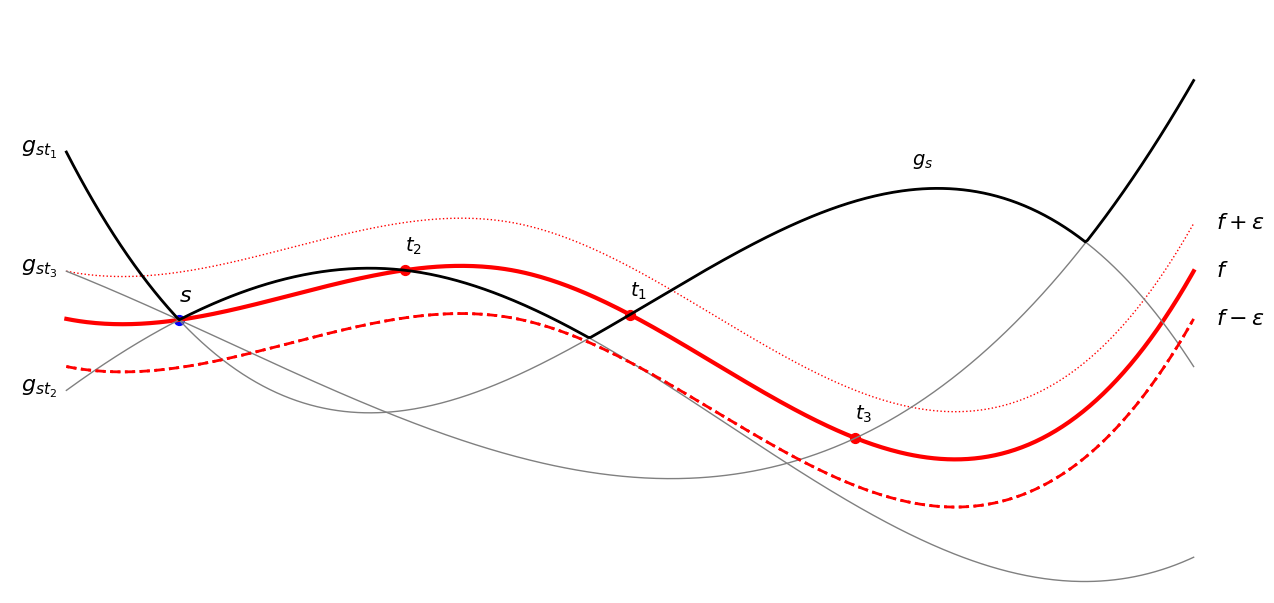
\includegraphics[width=1.0\textwidth]{./img/weierstrass_A_4.png}
            \caption{The construction of $g_s$. Here, we only required three points
            $T = \{t_1, t_2, t_3\}$.}
            \label{fig:weierstrass_A}
        \end{figure}

        We repeat this process again, this time to obtain an upper bound. For each $s
        \in K$, the continuity of $g_s$ means that there exists an open set $U_s
        \subseteq K$ such that \[
            g_s(x) < f(x) + \epsilon
        \] for all $x \in U_s$. Now, the collection of open sets $\{U_s\}_{s \in K}$
        covers the compact set $K$, hence we choose a finite sub-cover $\{U_s\}_{s
        \in S}$ where $S \subset K$ is finite. Define the function $g$ on $K$ as \[
            g = \min_{s \in S} g_s.
        \] Again, Theorem~\ref{theo:abs_max_min} gives $g \in \mathscr{B}$, and given
        $x \in K$, we can choose $s \in S$ such that $x \in U_s$, hence $g(x) \leq
        g_s(x) < f(x) + \epsilon$. Furthermore, every $g_s$ obeys $g_s(x) > f(x) -
        \epsilon$ everywhere; since $g$ is the minimum of finitely many functions,
        given $x \in K$ we find $s \in S$ such that $g(x) = g_s(x) > f(x) -
        \epsilon$. This shows that for all $x \in K$, \[
            f(x) - \epsilon < g(x) < f(x) + \epsilon,
        \] or $|g(x) - f(x)| < \epsilon$. Thus, $f$ is the uniform limit of functions
        in $\mathscr{B}$, proving that the uniform closure of $\mathscr{A}$ is the
        set $\mathscr{C}(K)$. \qedhere
        
        \begin{figure}[H]
            \centering
            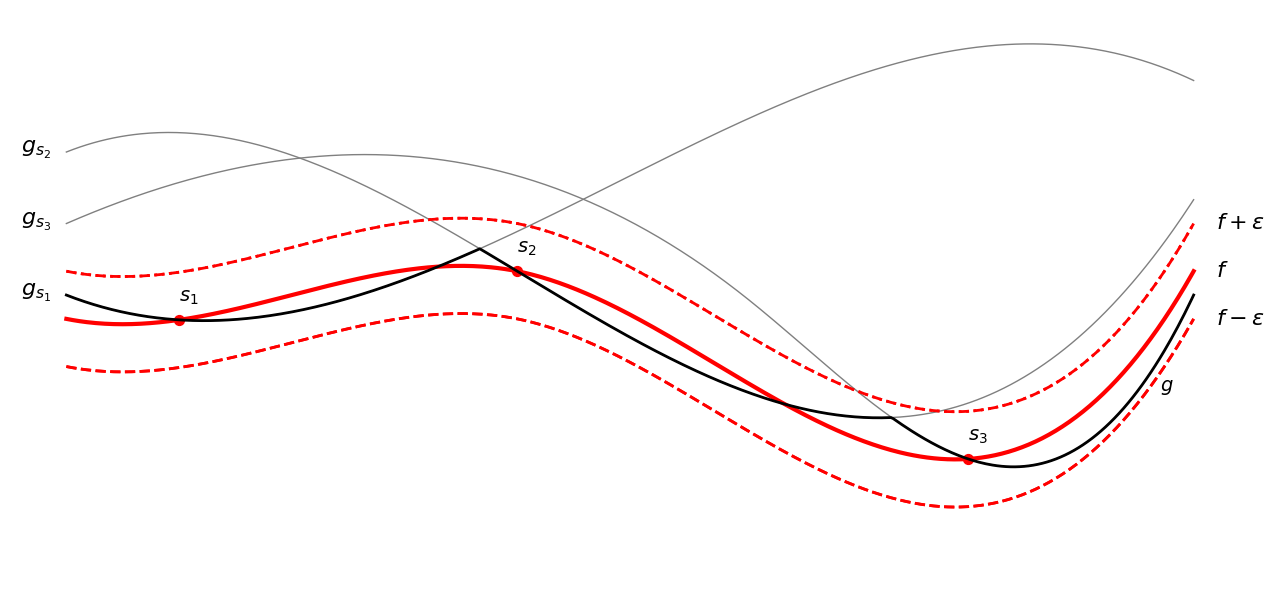
\includegraphics[width=1.0\textwidth]{./img/weierstrass_B_4.png}
            \caption{The construction of $g$. Again, we only required three points
            $S = \{s_1, s_2, s_3\}$.}
            \label{fig:weierstrass_B}
        \end{figure}
    \end{proof}

    \begin{corollary}
        Let $K$ be a compact subset of the Euclidean metric space $\R^n$, and let
        $\mathscr{P}$ be the algebra of polynomials in $n$ variables on $K$. Then,
        given any real valued, continuous function $f$ on $K$, there exists a
        sequence of polynomials $\{p_n\} \subset \mathscr{P}$ such that $p_n
        \to f$ uniformly on $K$.
    \end{corollary}
    \begin{proof}
        We need only check that $\mathscr{P}$ is an algebra of real continuous
        functions which separates points on $K$ and vanishes at no point of $K$,
        after which the result follows directly from the above theorem.

        Note that every polynomial function $p \in \mathscr{P}$ is of the form \[
            p(x) = \sum_{i_1, i_2, \dots, i_n} c_{i_1,i_2, \dots, i_n}
            x_1^{i_1}x_2^{i_2}\dots x_n^{i_n}.
        \] Each term in the finite sum is the product of projection maps $(x_1,
        \dots, x_n) \mapsto x_i$, which are continuous. Thus, the polynomial $p$ is
        indeed real valued and continuous, with the coefficients $c_{i_1 \dots i_n}
        \in \R$. It is evident that given a scalar $c\in \R$, we have $cp \in
        \mathscr{P}$ since the result is of the same form. Given $p, q \in
        \mathscr{P}$, it is also evident that $p + q \in \mathscr{P}$; term by term
        multiplication shows that $pq \in \mathscr{P}$ as well. Thus, $\mathscr{P}$
        is an algebra.

        To show that $\mathscr{P}$ vanishes nowhere on $K$, note that the constant
        polynomial $p(x_1, \dots, x_n) = 1 \neq 0$ on any $K \subseteq \R^n$. To show
        that $\mathscr{P}$ separates points on $K$, pick $y, w \in K$ where $y \neq
        w$. Then $y_j \neq w_j$ for at least one index $j$, so the polynomial $p(x_1,
        \dots, x_n) = x_j$ separates $w$ and $y$. Applying the Stone-Weierstrass
        Theorem completes the proof.
    \end{proof}

    \begin{corollary}
        Let $\mathscr{F}$ be the algebra of functions on $[0, \pi]$ of the form \[
            f(x) = a_0 + \sum_{n = 1}^N a_n \cos(nx) + b_n\sin(nx),
        \] for real coefficients $a_i, b_i$. Then, given any real valued, continuous
        function $f$ on $[0, \pi]$, there exists a sequence of functions $\{f_n\}
        \subset \mathscr{F}$ such that $f_n \to f$ uniformly on $[0,
        \pi]$.
    \end{corollary}
    \begin{proof}
        Like before, we need only check that $\mathscr{F}$ satisfies the requirements
        of the Stone-Weierstrass Theorem.

        It is clear that $\mathscr{F}$ is closed under sums and scalar multiples. To
        show that it is closed under products, we supply the following identities. \[
            \sin(nx)\sin(mn) = \frac{1}{2}\left[\cos((n - m)x) - \cos((n + m)x)
            \right],
        \] \[
            \sin(nx)\cos(mn) = \frac{1}{2}\left[\sin((n + m)x) + \sin((n - m)x)
            \right],
        \] \[
            \cos(nx)\cos(mn) = \frac{1}{2}\left[\cos((n + m)x) + \cos((n - m)x)
            \right].
        \] Thus, $\mathscr{F}$ is indeed an algebra. Now, $\mathscr{F}$ contains the
        constant function $x \mapsto 1$, hence $\mathscr{F}$ vanishes nowhere on
        $[0, \pi]$. Furthermore, given distinct $x_1, x_2 \in [0, \pi]$, we must have
        $\cos(x_1) \neq \cos(x_2)$, because the map $x \mapsto \cos(x)$ is strictly
        decreasing on $[0, \pi]$, and hence is injective. Thus, $\mathscr{F}$
        separates points on $[0, \pi]$.
    \end{proof}
    \begin{remark}
        Note that $\mathscr{F}$ does not separate the points $0$ and $2\pi$, due to
        the periodicity of the cosine and sine functions. In order to extend the
        domain to $[0, \pi\alpha]$, we may redefine $\mathscr{F}$ to consist of
        functions of the form \[
            f(x) = a_0 + \sum_{n = 1}^N a_n \cos(nx / \alpha) + b_n\sin(nx/\alpha).
        \] 
    \end{remark}
    \begin{remark}
        Instead, consider the unit circle $S^1$ (which is compact under the usual
        Euclidean topology on $\R^2$) as our domain. Let $\tilde{\mathscr{F}}$ be the
        algebra of functions of the form \[
            \tilde{f}(e^{ix}) = a_0 + \sum_{n = 1}^N a_n \cos(nx) + b_n\sin(nx).
        \] Here, we use the usual identification of $S^1$ with the unit circle in
        $\C$ described by the set of points satisfying $|z| = 1$. The closure of this
        algebra is the set of all real continuous functions on $S^1$, each of which
        can be identified with a unique real continuous, $\alpha$-periodic function
        on $\R$. \[
            \mathbb{I}\colon \mathscr{F} \to \tilde{\mathscr{F}}, \qquad
            f \mapsto \tilde{f}, \qquad
            \tilde{f}(e^{ix}) = f(\alpha x / 2\pi).
        \] Thus, given an arbitrary real valued, continuous function $f$ on $\R$ with
        period $\alpha$ and $\epsilon > 0$, pick $\tilde{g} \in \tilde{\mathscr{F}}$
        such that $|\tilde{g}(z) - \tilde{f}(z)| < \epsilon$ on $S^1$. Thus, for all
        $x \in \R$, we have \[
            |g(x) - f(x)| = |\tilde{g}(e^{2\pi ix / \alpha}) - \tilde{f}(e^{2\pi i x /
            \alpha})| < \epsilon.
        \] 
    \end{remark}

    \begin{theorem}
        Let $\mathscr{A}$ be an algebra on a compact metric space $K$ which satisfies
        the requirements of the Stone-Weierstrass Theorem. Then, given $f \in
        \mathscr{C}(K)$, there exists a monotonically decreasing sequence of
        functions from $\mathscr{A}$ which converge uniformly to $f$ on $K$.
    \end{theorem}
    \begin{proof}
        For all $n \in \N$, define the functions $f_n = f + 2 /3^{n}$ and use the
        Stone-Weierstrass theorem to select functions $g_n \in \mathscr{A}$ such that
        \[
            |g_n(x) - f_n(x)| < \frac{1}{3^n}
        \] everywhere on $K$. As a result, each $g_n$ satisfies \[
            f + \frac{1}{3^{n}} < g_n < f + \frac{1}{3^{n - 1}}
        \] on $K$. This immediately gives $g_n > g_{n + 1}$ for all $n \in \N$.
        Furthermore, for all $x \in K$, we have \[
            |g_n(x) - f(x)| < \frac{1}{3^{n - 1}} \to 0
        \] which establishes $g_n \to f$ uniformly on $K$ by
        Theorem~\ref{theo:uniform_M_n}.
    \end{proof}


\end{document}
% vim: set tabstop=4 shiftwidth=4 softtabstop=4:
